
%%% Local Variables:
%%% mode: latex
%%% TeX-master: t
%%% End:

\chapter{引言}
\label{chap:intro}

互联网与云计算的发展,越来越多的应用从本地迁移到云端,并涌现出大量新兴的互联网应用,
承载这些应用的数据中心成为了如同电力系统一样的社会基础设施。
与此同时,现代数据中心正在面临着权衡资源利用率与应用服务质量的挑战:
从应用开发者角度,服务质量是第一位的,因为它直接关系到用户体验与其收益,
由于互联网应用负载的波动性,开发人员通常会为自己的应用过量分配资源以满足峰值时的负载需求,
这造成了非常低的服务器利用率,通常只有6\%-12\%;
而对于数据中心运维人员,资源利用率直接反映其运维成本,虽然将不同应用混合部署到同一台服务器,
充分利用空闲时段的服务器资源可以有效提高数据中心利用率,
但多应用混合部署引入的软硬件资源共享会造成应用间无管理的资源竞争,
使得应用性能出现不可预测的波动,进而影响应用的服务质量。
由上可知,如何权衡数据中心资源利用率与应用服务质量是当前数据中心亟待解决的重要问题。

可以从三个角度解决这一问题:
其一是通过上层软件机制实现干扰容忍,在应用层保障服务质量,
如Google提出的Hedged Requests和Tied Requests方案\cite{dean_tail_2013},
通过向多个副本发送请求,并选择最快返回的结果以达到干扰容忍的目的;
R. Kapoor等人在文章\cite{Kapoor:2012:Chronos}中提出了Chronos架构,
以降低数据中心应用的长尾延迟;
另外一些工作\cite{timecard:2013, d2p:2014}尝试记录单个请求延迟在每个环节处理时间,
然后在分布式处理框架中传播,基于这些传播的信息来进行请求的处理与调度。
其二是在作业调度层次,通过profile的方式预测应用混合后的干扰情况,
将相互之间干扰较小的应用部署到同一台服务器\cite{mars_bubble-up:_2011, kambadur_measuring_2012}。
其三是提供一个良好的隔离环境,降低由资源竞争所产生的应用间干扰,
可以在各个层次实现隔离,
如数据中心作业调度层\cite{Hindman:2011:Mesos, Schwarzkopf_omega_2013, borg:2015}、
操作系统\cite{cgroup, lin_gaining_2008, tam_managing_2007, liu_software_2012, Liu:2014:ISCA}、
虚拟化层\cite{Xu:2013:Bobtail:, Xu:2013:SMALL}、
硬件\cite{kasture_ubik:_2014, sanchez_vantage:_2011, sanchez_zcache:_2010, qureshi_utility-based_2006, muralidhara_reducing_2011}等。


其中前两种方案在实施时需要对目标应用具有非常深入的理解:
方案一需要对应用架构与实现细节进行修改,以达到应用层干扰容忍的目的;
方案二虽然无需对应用进行修改,但需要对应用的资源占用以及不同应用之间的干扰状况进行分析,
才能得到最优的调度方案。
当应用数量不多且有条件进行以上所述的分析或修改,通过精细的应用架构设计与调度机制,
可以有效的解决前文所提到的资源利用率与服务质量相冲突的问题。
但在现实数据中心特别是云计算数据中心内,以上假设并不成立。

首先,数据中心内通常会运行大量的应用,
如Google的数据\cite{Reiss_googletrace_2012}表明其数据中心在两个月内累计运行超过2,000,000个应用,
无论是改造这些应用或是对应用之间的干扰行为进行分析都是不可行的。
即使只对部分关键的应用进行改造使其适应干扰环境,
云计算环境下的``吵闹的邻居(Noisy Neighbors)''也会使这些努力的结效果大打折扣。

其次,调度方案无法解决短时运行的干扰应用对其他正常应用带来的影响,特别是随着DevOps的兴起,
由于开发调试与线上部署是不断迭代进行的,调试过程中所引入的短时干扰应用数量大大增加,
Google的数据\cite{Reiss_googletrace_2012}发现大量的小于6分钟的应用都是来自于这些调试应用。
当调度器发现干扰并准备采取调度措施时干扰应用可能已经结束,同时新的干扰应用又开始运行,并带来新的干扰。

对于第三种隔离方案,
单纯软件层次的隔离只能做到较粗粒度的资源管理,实现的效果有限;
同时应用的不同特征造成资源竞争点是分布在整个软件栈中,
因此只能根据实际场景做针对性的优化;
再次,在如此复杂的软件栈中找到真正的资源竞争点需要大量的时间与精力,
这同样不能满足云计算的场景下应用多样与快速部署的需求。
除了软件栈上的共享,混合部署的应用在硬件层次上也存在大量的共享,
如共享末级缓存、内存控制器、I/O等,
上文所提到的这些研究专注于如何在这些共享硬件上提供隔离功能,
但这些研究大都只关注于一种类型的资源,而且是针对特定的场景,
因此缺少灵活的软件编程接口,不能适用于通用的计算场景。

综上可知,
现有的三种方案都不能很好的解决当前云计算数据中心中遇到的资源利用率与服务质量矛盾的问题,
该问题的本质是为应用提供区分化服务,
而如何解决目前计算机系统的软硬件资源的无管理共享状态是实现区分化服务的关键。
现有研究在一定程度上能够解决软件层次的共享管理问题,
但无管理的硬件共享使得该问题并没有被完全解决。
造成这一现状的原因是目前的计算机体系结构在设计时并没有考虑到多应用共享场景,
其指令集抽象不足以将上层应用需求传递到下层硬件,
在不能区分应用需求的前提下很难做到区分化服务。
软件层次已有很多方案可以用于区分不同应用,如操作系统级的进程PID或cgroup,
或更细粒度的应用级标签\cite{timecard:2013,d2p:2014, mesnier_differentiated_2011, thereska_ioflow:_2013}。
硬件层次也需要一种应用需求传递机制,
正如``21st Century Computer Architecture''白皮书中所提出的:

\begin{quotation} 
\emph{\textbf{Better Interfaces for High-Level Information.}
Current ISAs fail to provide an efficient means of capturing software-intent or conveying critical high-level information to the hardware.
For example, they have no way of specifying when a program requires energy efficiency, robust security, or a desired Quality of Service (QoS) level.
Instead, current hardware must try to glean some of this information on its own ......
\textbf{New, higher-level interfaces are needed to encapsulate and convey programmer and compiler knowledge to the hardware,}
resulting in major efficiency gains and valuable new functionality.}\cite{21st_architecture}
\end{quotation}

因此,我们需要为数据中心计算机设计一种新的体系结构,
使其能够从硬件上改变资源的``无管理共享''现状以,
从体系结构上支持应用服务质量保障,
在此基础上实现数据中心资源根据应用动态管理以提高资源利用率。

\begin{figure}[H]
  \centering
  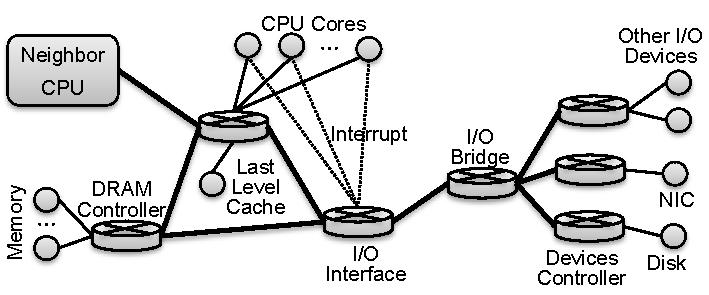
\includegraphics[height=4cm]{intro/computer-as-a-network.pdf}
  \caption[计算机内部本质是一个网络]{
    计算机内部部件之间以数据包(packet)进行通信,比如
    处理器核之间使用基于包的片上网络、
    处理器之间采用基于包的互连协议(如QPI和HT)、
    I/O设备与内存之间则通过PCI-E包进行通信。
    因此,计算机本身即可视为一个网络。}
  \label{fig:computer-as-a-network}
\end{figure}

基于以上需求,
本文提出了一种新体系结构:资源按需管理可编程的体系结构PARD\cite{pard:2015},
使数据中心服务器能够支持区分化服务,通过细粒度的硬件资源管理以及灵活的编程接口,
实现在保障关键应用服务质量的前提下提高服务器资源利用率。
PARD体系结构的核心是基于一个重要的观察:\textbf{计算机内部本质上是一个网络}。
如图\ref{fig:computer-as-a-network}所示,
CPU核、共享缓存、内存控制器、I/O设备等可以被看做是网络节点,它们之间通过包进行通信;
除了处理请求以外,这些``网络节点''与网络中的路由器/交换机具有相似的请求转发功能。
在网络领域,如何实现端到端的服务质量保障已有大量的研究,并已形成标准。
如IETF(Internet Engineering Task Force, 互联网工程任务组)于1998年提出了区分化服务
(Differentiated Services)\cite{DiffServ}的概念,
如今区分化服务已经成为应用最广泛的服务质量保障机制之一;
软件定义网络(SDN)\cite{SDN}的出现,进一步促进了网络领域服务质量保障的发展,其提出的
(1)控制平面与数据平面分离,和(2)集中控制的统一编程接口,
为网络管理带来了极大的灵活性。
本文希望能够将网络领域的区分化服务和软件定义网络的思想应用到计算机内部的网络,
用以解决数据中心当前面临的资源利用率与应用服务质量矛盾。

然而相比在计算机网络,
在体系结构这一``内部网络''中实现区分化服务与软件定义网络的功能需要面临一些额外的挑战:

首先,网络栈是整个网络中产生数据包的唯一位置,因此可以很容易的在其中增加标签机制,
实现网络流的区分。
而在计算机中有大量不同类型的硬件部件都能够向``内部网络''发送请求,
而且这些请求的类型各不相同,
如何为这些来自于不同硬件部件、类型各异的请求增加应用标签是需要解决的第一个挑战。

其次,与网络中交换机或路由器这些只进行存储转发的网络设备不同,
计算机内各个硬件部件通常包含更为复杂的功能,
如:处理器末级缓存需要为请求除完成将请求转发到下层内存控制器外,
还需要决定哪些请求数据缓存在本地,以及替换哪些数据到内存控制器;
内存控制器需要进行复杂的地址映射实现将物理地址映射到DRAM芯片,
同时还需要实现调度策略以提高访存性能;其他一些I/O设备具有更为复杂的功能。
因此如何为这些不同类型的硬件部分提供一个统一的控制平面实现对硬件资源的管理是第二个挑战。

最后,在交换机或路由器中已经为管理员提供了访问和配置其控制平面的固件接口,
而在当前的计算机中并没有类似的的固件接口。
服务器中普遍配置的IPMI/BMC\cite{ipmi}提供了诸如温度监控、电源控制、
BIOS访问等有限的监控与管理功能,利用该模块
如何实现硬件控制平面的管理,以及如何为用户(管理员)提供灵活的访问与编程接口是面临的第三个挑战。

为了解决以上三个挑战,PARD体系结构的核心设计理念可以归结为以下四点:
\textbf{1)标签机制},
通过在请求源(如处理器核或具有DMA功能的I/O设备)增加标签寄存器,使用其记录当前正在使用该部件的应用标签,
发出请求时附带该标签,并随着请求在整个计算机内部传播,实现应用区分;
\textbf{2)可编程控制平面},
为共享硬件资源的控制器增加控制平面,控制平面可根据请求标签查询规则进行区分处理,该规则可通过软件实现可编程;
\textbf{3)节点内统一资源管理},
节点内所有的控制平面通过控制平面网络连接到资源管理模块,提供对控制平面的编程接口,实现所有共享资源的统一管理;
\textbf{4)Trigger$\Rightarrow$Action编程方法},
一种基于动作触发的资源管理策略,实现资源实时监控和调整。

本文后续章节将讨论如何在现有体系结构上扩展以实现标签机制;
通用控制平面的设计以及可编程机制的实现,
并包括末级缓存控制器和内存控制器中控制平面的具体设计;
基于以上两种机制实现无Hypervisor的全硬件支持虚拟化系统,
以及如何实现资源按需分配的区分化服务,并使用模拟器对其效果进行验证。
最后在基于FPGA的原型系统中验证PARD体系结构的效果,
并讨论了原型系统实现过程中的经验与教训。


\section{本文的主要贡献}

本文的论点是:
在应用数量众多、需求多样且不断变化的数据中心场景下,计算机体系结构需要重新设计,
为应用提供区分化服务、良好的性能隔离,并具备灵活的资源管理编程接口,
实现资源使用的强控制与按需分配,
才能解决数据中心资源利用率与服务质量冲突的问题。

本文的主要贡献包括:

% 可在多个层次(虚拟机、进程、线程、API、...)区分应用,实现了NoHyper功能
第一,提出``标签化地址空间(Labeled Address Space)''概念。
正如多进程技术的出现引入了虚拟地址空间抽象,
随着虚拟化、云计算与多租户使用模式的出现,
现有的虚拟地址空间抽象无法满足多租户之间的隔离需求,
一些硬件隔离技术如EPT、I/O MMU、SR-IOV等试图在现有的体系结构下支持隔离需求,
其本质则是在虚拟地址空间外增加一层额外的地址空间,但这些技术只是在功能层面上实现了隔离,
而与性能相关的部件如共享末级缓存、内存控制器等在现有体系结构下并没有实现隔离。
本文提出的标签化地址空间抽象,使用统一标签区分不同应用,
并为计算机系统内所有请求标识应用标签,硬件不再需要通过猜测的方式区分应用,
而是通过标签机制打破目前体系结构中软硬件之间的语言鸿沟,
使得共享的硬件资源能够区分来自不同应用的请求并进行区分处理。
%可在不同层次实现应用区分,如虚拟机、进程、线程或使用API标识的数据/代码段,
%以实现不同粒度的区分化服务。
%以虚拟机粒度为例,通过标签机制以及共享硬件资源内部基于标签的划分机制,
%可将一台计算机划分为多台独立的逻辑域(Logical Domain),
%在每个逻辑域内独立运行操作系统,实现NoHyper\cite{keller_nohype:_2010}的功能。

% 表+Trigger/Action <=> 处理器方案
第二,提出硬件资源共享管理方法,为硬件资源共享提供配置、监控、反馈功能,
实现毫秒(ms)级的性能反馈。
%本文两个重要观点是:资源监控与管理结合,共享资源本地与全局协同管理结合。
实时的监控与反馈是实现细粒度资源管理的重要前提,软件监控方案无法满足实时性的需求,
在硬件上直接实现监控与反馈,提出使用通用的``控制平面''实现硬件资源的配置与监控。
在具体实现上,通过基于表的控制平面实现通用的硬件资源管理接口,
使用基于处理器的数据平面实现硬件请求的灵活控制,
为计算机系统实现硬件资源可管理提供支持。

第三,提出节点内硬件共享资源的协同管理。
控制平面构成了计算机系统内硬件资源管理的基本单元,由于硬件资源之间具有关联性,
需要进行全局统筹管理。
本文通过使用控制面网络将节点内所有的控制平面连接到集中式的资源管理模块,
对硬件共享资源进行协同管理。

以上三点贡献已在PARD的模拟器及FPGA原型系统中实现。
模拟器原型是基于gem5\cite{binkert_gem5_2011}实现的全系统时钟精确模拟器,
增加或修改了大约24,118行C++/Python代码,该模拟器以在LGPL协议下开源
\footnote{PARD-gem5模拟器开源地址https://github.com/fsg-ict/PARD-gem5}。
FPGA原型系统基于MicroBlaze系统在Xilinx VC709开发板实现并完成验证,
系统运行在133MHz频率,包含4个处理器核。
两个原型系统可以作为后续相关研究的参考平台。


\section{论文的组织}

\begin{figure}[htb]
  \centering
  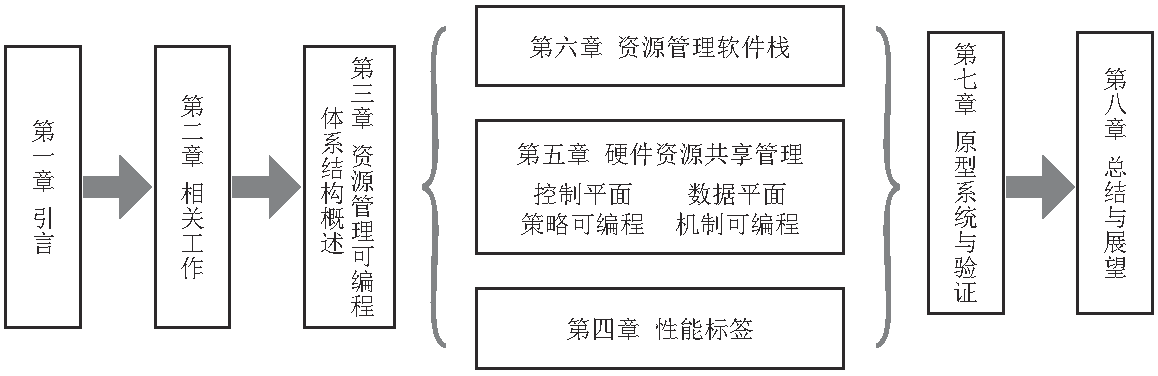
\includegraphics[width=\textwidth]{intro/thesis-structure}
  \caption{本文内容与组织结构}
  \label{fig:thesis-structure}
\end{figure}

本文共分八章,组织结构如图\ref{fig:thesis-structure}所示。

第二章介绍数据中心面临的资源利用率与服务质量冲突问题的挑战,
然后讨论现有数据中心技术的局限性,
并介绍解决该问题的现有研究。

第三章介绍PARD体系结构与关键特性,
并讨论如何利用PARD所提供的特性解决应用服务质量与资源利用率相冲突的问题。

第四章介绍PARD体系结构的基础标签化地址空间,
讨论在现有体系结构下实现标签化地址空间需要解决的关键问题,
并在模拟器上通过标签化地址空间改造,实现无软件支持的全硬件虚拟化功能。

第五章讨论硬件共享资源的管理方法,包括硬件资源的控制平面/数据平面抽象,
同时以共享末级缓存和内存控制器为例,讨论控制平面与数据平面的设计,
并通过模拟的方式验证该方案的有效性。

第六章介绍资源管理模块与资源协同管理相关的内容,包含节点内资源统一管理,
以及如何将PARD集成到现有的数据中心管理系统中(以Mesos\cite{Hindman:2011:Mesos}为例)。

第七章基于前四章的设计给出本文资源管理可编程体系结构的FPGA原型系统实现,
并对原型系统各部分功能的正确性、性能与开销进行评测。

第八章总结全文并介绍未来可能的研究工作。

